\documentclass[12pt,a4paper]{report}

\usepackage[margin=1in]{geometry}
\usepackage{graphicx}
\usepackage{float}
\usepackage{array}
\usepackage{booktabs}
\usepackage{tikz}
\usepackage{listings}
\usepackage{xcolor}
\usepackage{hyperref}
\usepackage{setspace}

\onehalfspacing
\graphicspath{{./}}

\hypersetup{
    colorlinks=true,
    linkcolor=black,
    urlcolor=blue
}

\lstset{
    basicstyle=\ttfamily\small,
    breaklines=true,
    frame=single,
    columns=fullflexible,
    backgroundcolor=\color{gray!8}
}

\begin{document}

\begin{titlepage}
    \centering
    \vspace*{0.5cm}
    {\Large \textbf{SSN College of Engineering}}\\[0.3cm]
    {\large Department of Computer Science and Engineering}\\[1.2cm]

    {\Large \textbf{Compiler Design Laboratory}}\\[0.4cm]
    {\large \textbf{Experiment 10}}\\[1.2cm]

    {\LARGE \textbf{Implementation of a Compiler for a Source Program}}\\[0.3cm]
    {\Large \textbf{Cross Compiler Platform}}\\[1.4cm]

    \begin{tabular}{>{\bfseries}l l}
        Name: & \underline{\hspace{7cm}}\\[0.35cm]
        Register Number: & \underline{\hspace{7cm}}\\[0.35cm]
        Semester / Section: & \underline{\hspace{7cm}}\\[0.35cm]
        Subject Code: & \underline{\hspace{7cm}}\\[0.35cm]
        Date: & \underline{\hspace{7cm}}\\
    \end{tabular}

    \vfill
    {\large Academic Year 2026--2027}
\end{titlepage}

\chapter*{Certificate}
This is to certify that the mini project titled \textbf{``Cross Compiler Platform''} has been developed as part of the Compiler Design Laboratory experiment. The project accepts a simple source program, performs lexical analysis, syntax analysis, semantic analysis, intermediate code generation, optimization, and target code generation for multiple target platforms.

\vspace{2cm}
\begin{tabular}{p{0.45\textwidth} p{0.45\textwidth}}
    \centering Student Signature & \centering Faculty Signature
\end{tabular}

\tableofcontents
\newpage

\chapter{Introduction}
A compiler is a system software tool that translates a program written in a source language into an equivalent program in a target language. A cross compiler is a special type of compiler that runs on one platform but generates code for another platform. This project implements a small cross compiler platform for a simple programming language and demonstrates each phase of compilation through a browser-based user interface.

\section{Aim}
To design and develop a cross compiler platform that accepts a source program written in a simple language and performs lexical analysis, syntax analysis, semantic analysis, AST generation, intermediate code generation, code optimization, and target code generation for multiple target platforms.

\section{Objectives}
\begin{itemize}
    \item To accept a source program through a user interface.
    \item To display the tokens generated during lexical analysis.
    \item To validate the grammar during syntax analysis.
    \item To perform semantic analysis using a symbol table.
    \item To generate an Abstract Syntax Tree.
    \item To generate Three Address Code.
    \item To apply a code optimization technique.
    \item To generate target code for C, ARM Assembly, and RISC-V Assembly.
    \item To demonstrate execution output wherever supported.
\end{itemize}

\chapter{Task 1: Familiarization of Cross Compiler}
A cross compiler is a compiler that executes on one machine or platform, called the host platform, but produces object code or target code for another machine or platform, called the target platform. For example, a compiler running on a Windows system may generate ARM assembly code for an embedded processor. This is different from a native compiler, where the compiler runs on the same platform for which it generates code.

Cross compilers are widely used in embedded systems, operating system development, mobile application development, and processor simulation environments. They allow developers to write and compile programs on powerful host machines while producing executable code for smaller or different target devices.

In this project, the compiler platform accepts a small C-like source language and generates target code for more than one platform. The compiler performs standard phases such as lexical analysis, syntax analysis, semantic analysis, AST generation, intermediate code generation, optimization, and target code generation.

\section{T-Diagram Illustration}
The T-diagram represents the relationship between the source language, implementation platform, and target language of a compiler.

\begin{figure}[H]
    \centering
    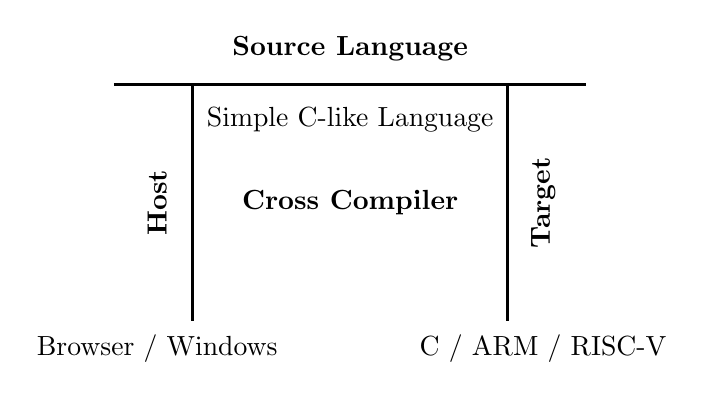
\begin{tikzpicture}[line width=1pt]
        \draw (0,0) -- (6,0);
        \draw (1,0) -- (1,-3);
        \draw (5,0) -- (5,-3);
        \node at (3,0.45) {\textbf{Source Language}};
        \node at (3,-0.45) {Simple C-like Language};
        \node[rotate=90] at (0.55,-1.5) {\textbf{Host}};
        \node[rotate=90] at (5.45,-1.5) {\textbf{Target}};
        \node at (3,-1.5) {\textbf{Cross Compiler}};
        \node at (0.55,-3.35) {Browser / Windows};
        \node at (5.45,-3.35) {C / ARM / RISC-V};
    \end{tikzpicture}
    \caption{T-diagram of the cross compiler platform}
\end{figure}

\section{Example}
If the source program is:

\begin{lstlisting}
int a = 10;
int b = 20;
int c;
c = a + b * 2;
print c;
\end{lstlisting}

The compiler can generate optimized C target code as:

\begin{lstlisting}[language=C]
#include <stdio.h>

int main() {
  int a, b, c;
  int t1, t2;
  a = 10;
  b = 20;
  t1 = 40;
  t2 = 50;
  c = 50;
  printf("%d\n", 50);
  return 0;
}
\end{lstlisting}

\chapter{System Design}
\section{Source Language}
The source language supports integer declarations, assignment statements, arithmetic expressions, and print statements.

\begin{lstlisting}
declaration: int id;
declaration: int id = expression;
assignment : id = expression;
print      : print expression;
expression : expression + term | expression - term | term
term       : term * factor | term / factor | factor
factor     : number | identifier | ( expression )
\end{lstlisting}

\section{Compiler Phases}
\begin{enumerate}
    \item \textbf{Lexical Analysis:} Converts source code into tokens.
    \item \textbf{Syntax Analysis:} Checks whether the token sequence follows grammar rules.
    \item \textbf{Semantic Analysis:} Uses a symbol table to validate declarations and variable usage.
    \item \textbf{AST Generation:} Produces a tree representation of the program structure.
    \item \textbf{Intermediate Code Generation:} Generates Three Address Code.
    \item \textbf{Optimization:} Applies constant folding and constant propagation.
    \item \textbf{Target Code Generation:} Produces C, ARM Assembly, and RISC-V Assembly output.
\end{enumerate}

\section{Use of Lex/Flex and Yacc/Bison}
The project includes Flex and Bison specification files for scanner and parser construction. Flex is used to define token patterns, while Bison is used to define grammar rules and parser actions. These files are included in the project source under the \texttt{flex-bison} directory.

\chapter{Implementation}
\section{Lexical Analysis}
The lexical analyzer identifies keywords, identifiers, numbers, operators, parentheses, assignment operators, and semicolons. Invalid characters are reported as lexical errors.

\section{Syntax Analysis}
The syntax analyzer verifies the structure of declarations, assignments, print statements, and arithmetic expressions. Syntax errors are displayed if the source program does not match the grammar.

\section{Semantic Analysis}
The semantic analyzer builds a symbol table and checks whether identifiers are declared before use. It also reports duplicate declarations and undeclared variable usage.

\section{Intermediate Code and Optimization}
The compiler generates Three Address Code for expressions and statements. Constant folding is applied to replace expressions involving only constants with their computed values.

\section{Target Code Generation}
The platform generates target code for:
\begin{itemize}
    \item C language
    \item ARM-style assembly
    \item RISC-V-style assembly
\end{itemize}

\chapter{Output Screenshots}
\begin{figure}[H]
    \centering
    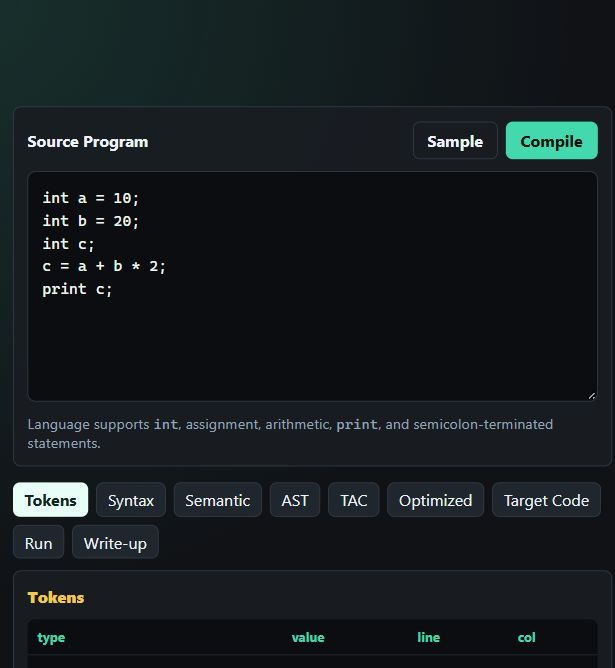
\includegraphics[width=\textwidth]{img1.png}
    \caption{Lexical analysis output, source program, compiler flow, and symbol table}
\end{figure}

\begin{figure}[H]
    \centering
    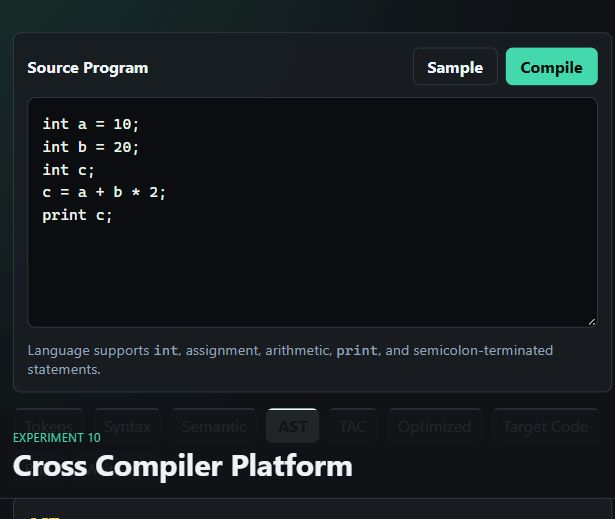
\includegraphics[width=\textwidth]{img2.png}
    \caption{Abstract Syntax Tree generated by the compiler}
\end{figure}

\begin{figure}[H]
    \centering
    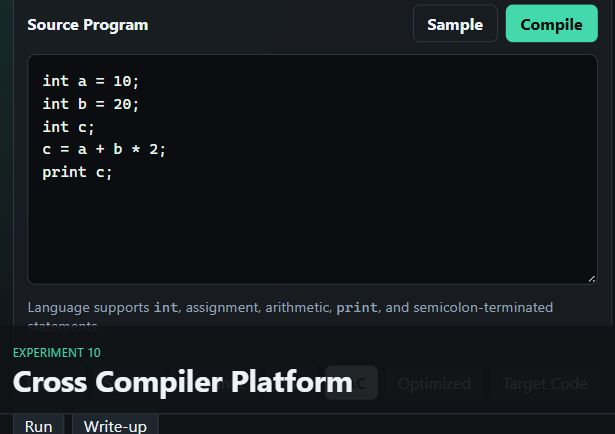
\includegraphics[width=\textwidth]{img3.png}
    \caption{Three Address Code generated from the source program}
\end{figure}

\begin{figure}[H]
    \centering
    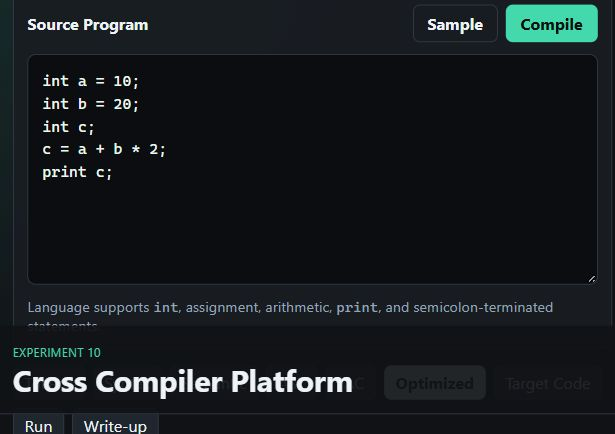
\includegraphics[width=\textwidth]{img4.png}
    \caption{Optimized intermediate code after constant folding}
\end{figure}

\begin{figure}[H]
    \centering
    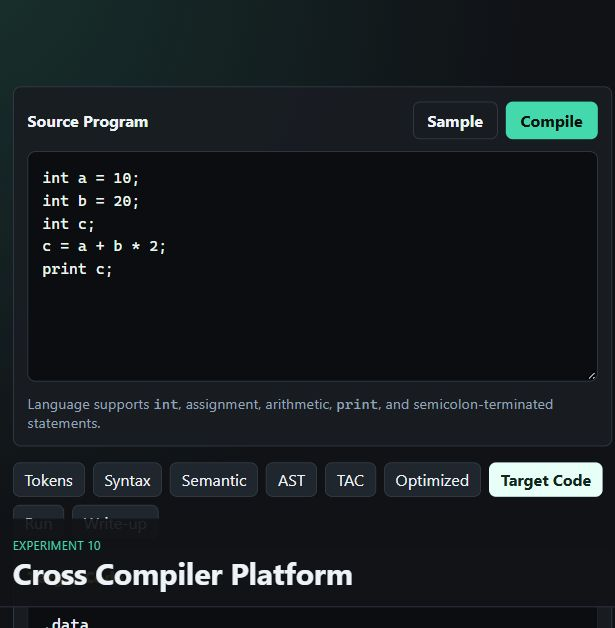
\includegraphics[width=\textwidth]{img5.png}
    \caption{Generated ARM target code}
\end{figure}

\chapter{Result}
The cross compiler platform was successfully designed and implemented. It accepts a simple source program, performs all major compiler phases, displays tokens, syntax result, semantic result, symbol table, AST, TAC, optimized TAC, generated target code, and simulated output. Target code generation was demonstrated for C, ARM Assembly, and RISC-V Assembly.

\chapter{Conclusion}
This mini project demonstrates the complete workflow of a cross compiler. It shows how a source program is processed through lexical, syntax, and semantic analysis before being converted into intermediate code and optimized target code. The visual user interface makes each compiler phase easier to understand, while the included Flex and Bison files satisfy the scanner and parser implementation requirement.

\appendix
\chapter{Sample Source Program}
\begin{lstlisting}
int a = 10;
int b = 20;
int c;
c = a + b * 2;
print c;
\end{lstlisting}

\chapter{Sample Flex Token Rules}
\begin{lstlisting}
"int"               { return INT; }
"print"             { return PRINT; }
[0-9]+              { yylval.num = atoi(yytext); return NUMBER; }
[A-Za-z_][A-Za-z0-9_]* { yylval.id = strdup(yytext); return ID; }
"="                 { return ASSIGN; }
"+"                 { return PLUS; }
"-"                 { return MINUS; }
"*"                 { return STAR; }
"/"                 { return SLASH; }
";"                 { return SEMICOLON; }
\end{lstlisting}

\chapter{Sample Bison Grammar Rules}
\begin{lstlisting}
statement:
    INT ID SEMICOLON
  | INT ID ASSIGN expr SEMICOLON
  | ID ASSIGN expr SEMICOLON
  | PRINT expr SEMICOLON
  ;

expr:
    expr PLUS term
  | expr MINUS term
  | term
  ;
\end{lstlisting}

\end{document}
